\placelogofalse
\begin{frame}{Classic CFD}
\begin{columns}
\column{0.48\linewidth}
\begin{outline}
\1 Discretize space into control Volumes 
\1 Solve for macroscopic fluid values
\1 Common to require global solve for pressure term
\end{outline}

\column{0.48\linewidth}
\centering
\begin{center}
\textbf{Conservation of Mass}
\begin{align*}
  \frac{\partial \rho}{\partial t} + \nabla \cdot (\rho \bm{u}) &= 0 \\
\end{align*}
\textbf{Conservation of Momentum}
\begin{align*}
\frac{\partial}{\partial t} (\rho \bm{u}) 
+ \nabla \cdot (\rho \bm{u} \times \bm{u}) &= 
- \nabla \bm{p} + \nabla \cdot \sigma
\end{align*}
  \includegraphics[width=0.8\linewidth]{FVM.png}
\end{center}
\placelogotrue

\end{columns}
\blfootnote{Figure from \href{https://www.researchgate.net/figure/Schematic-representation-of-an-FVM-model-FVM-finite-volume-method_fig5_347307910}{ResearchGate}}
\end{frame}

\placelogofalse
\begin{frame}{Lattice Boltzmann method (LBM): Discretization}
\begin{columns}
\column{0.58\linewidth}
\begin{outline}
\1 Model microscopic particles
\1 Recover macroscopic properties
\1 $D$ dimensional grid of points $x$
\2 Particle position distribution
\1 $Q$ dimensional ``lattice'' at each point
\2 Particle velocity distribution $f(x, \xi, t)$
\2 Directions $c_i$
\textit{streaming} and \textit{collision}
\end{outline}

\column{0.38\linewidth}
\centering
\begin{center}
  \includegraphics[width=0.9\linewidth]{lattice_figure.png}
  (a) D2Q9 (b) D3Q27
\end{center}
\end{columns}
\begin{align*}
  c_i &= \left\{
  \begin{array}{l l}
  (0, 0, 0) & i = 0\\
  (\pm 1, 0, 0), (0, \pm 1, 0), (0, 0, \pm) & i = 1,\ldots, 6\\
  (\pm 1, \pm 1, 0), (\pm 1, 0, \pm 1), (0, \pm 1, \pm 1)
                                            & i = 7, \ldots, 18 \\
  (\pm 1, \pm 1, \pm 1) & i = 19, \ldots, 26
  \end{array}
  \right.
\end{align*}
\blfootnote{Figure from \cite{Li2020}}
\end{frame}
\placelogotrue


\placelogofalse
\begin{frame}{LBM Theory Primer}
\begin{columns}
\column{0.48\linewidth}
\begin{outline}
\1 Lattice Boltzmann equation
\1 $f(x, t)$ approximates $\xi$
\1 Hermite Polynomial Basis \cite{De2019}
\2 Quadrature Rule with $c_i$.
\1 Collision operator, $\Omega$
\2 Relax towards equilibrium $f_{eq}$
\1 Moments of $f$ are macroscopic quantities 
\1 Advance time with two operators, 
\textit{streaming} and \textit{collision}
\end{outline}
\column{0.48\linewidth}
\centering
\begin{center}
  \begin{align*}
  \partial_t f(x, \xi, t)  + \xi \cdot \nabla f(x, \xi, t) = \Omega (f)
  \end{align*}

  \begin{align*}
  \rho(x, t) &= \sum_{i = 0}^{Q - 1} f_i(x, t) \\
  \rho(x,t)u(x,t) &= \sum_{i = 0}^{Q - 1}c_i f_i(x, t)
  \end{align*}
\end{center}
\end{columns}
\blfootnote{Figure from \cite{Li2020}}
\end{frame}
\placelogotrue

\begin{frame}{Streaming}
\begin{columns}
\column{0.48\linewidth}
\begin{outline}
\1 Non-local operator (Transport)
\1 Particles stream to next point in grid 
\1 Information travels at speed of sound!
\end{outline}
\begin{align*}
  f^{*}_i(x, t) &= f_i(x - c_i, t) 
\end{align*}
\column{0.48\linewidth}
\centering
  \begin{center}
    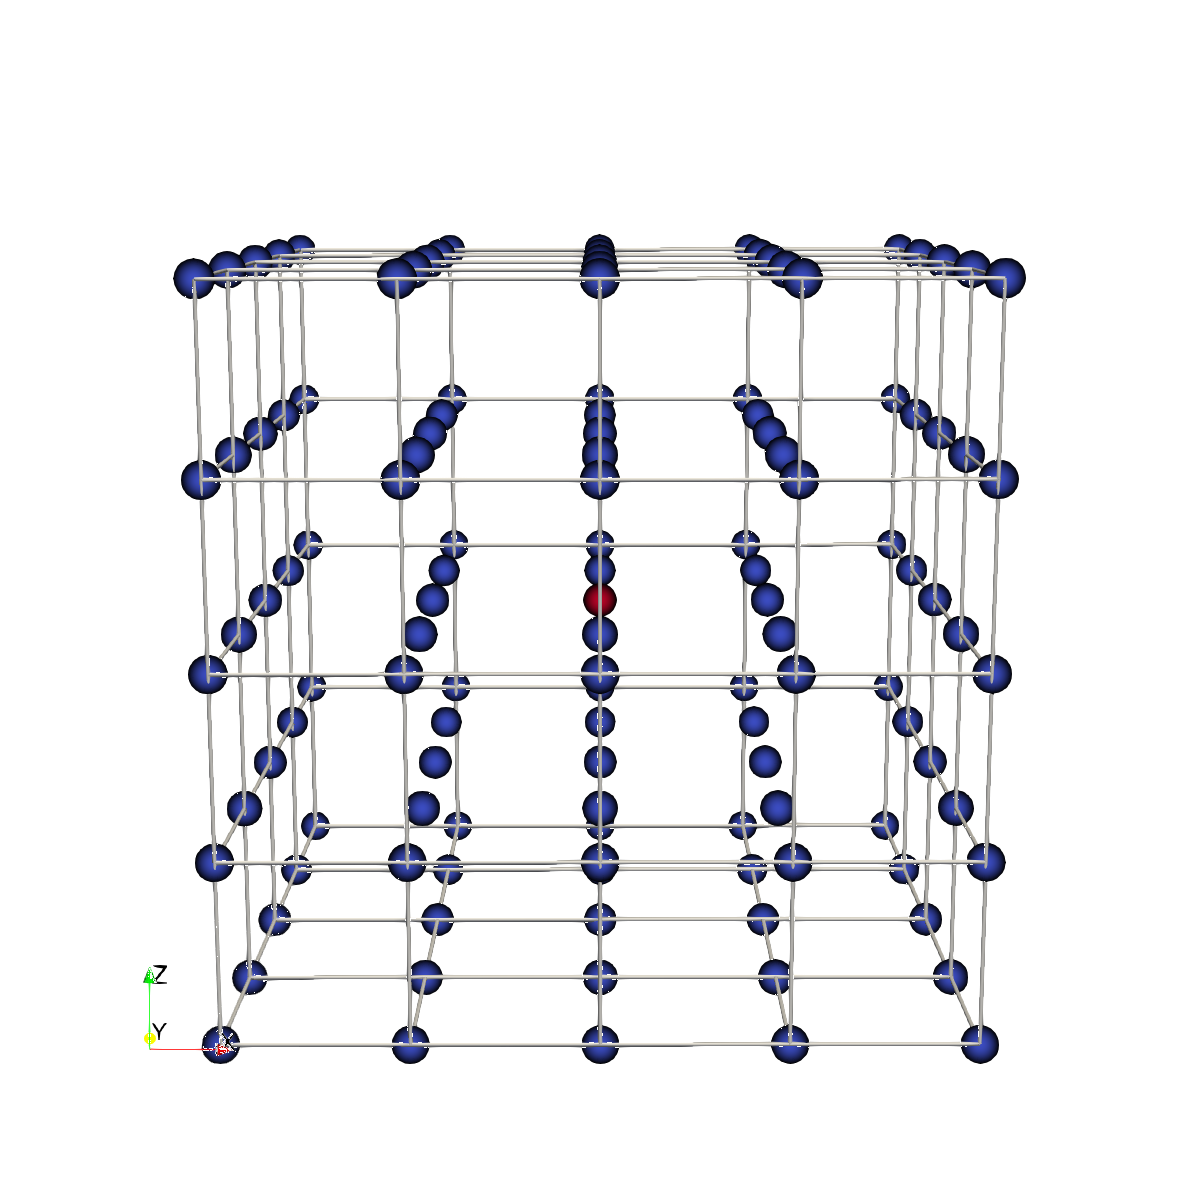
\includegraphics[width=0.4\linewidth]{stream_0.png}
    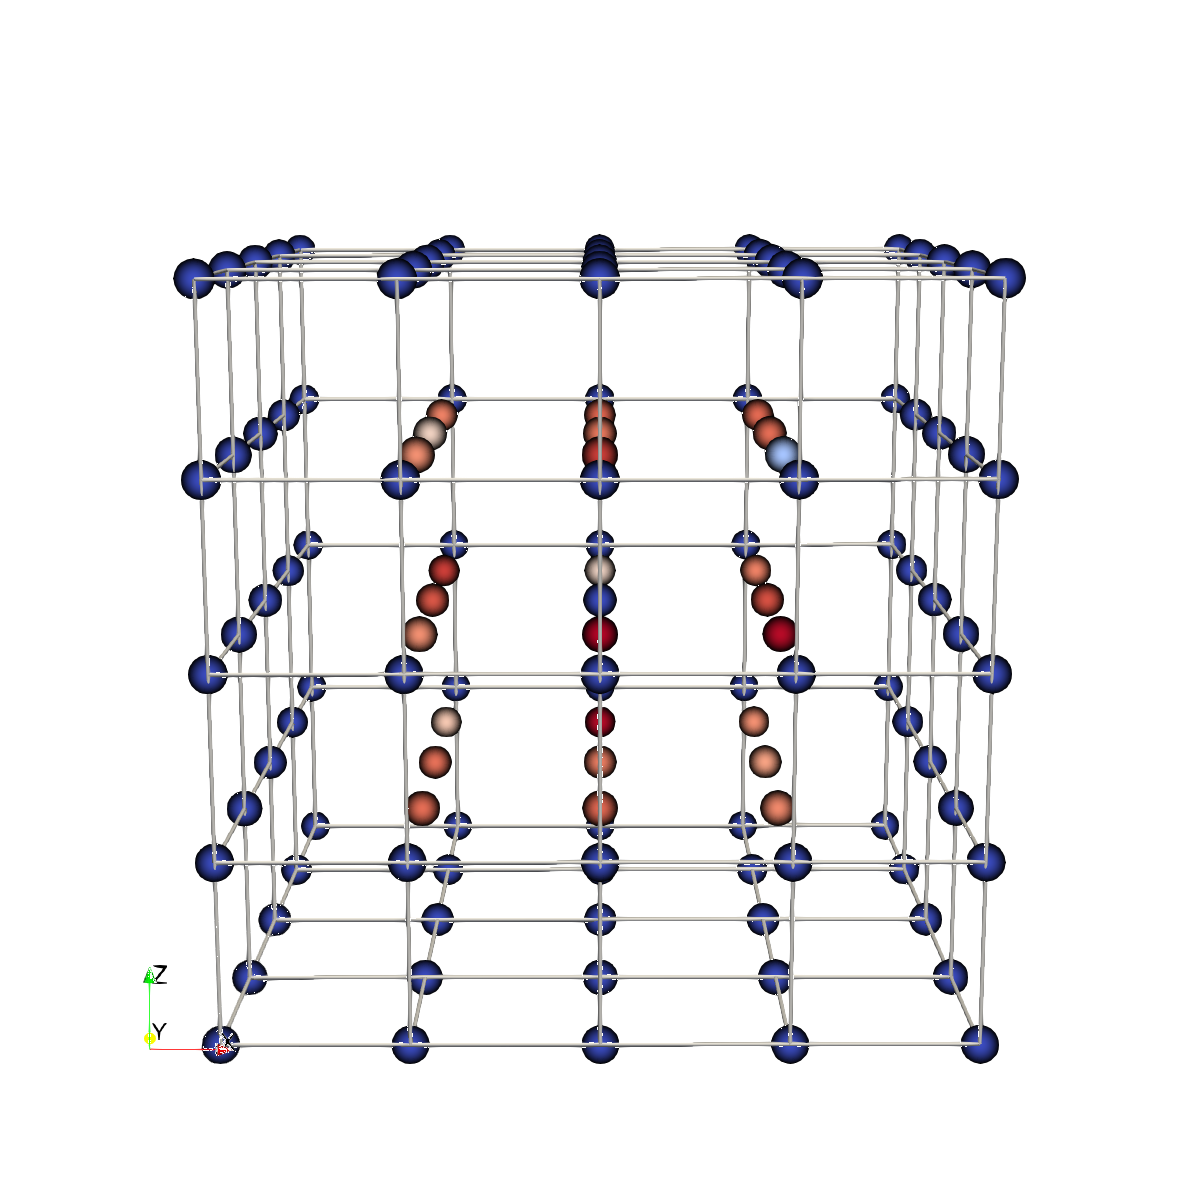
\includegraphics[width=0.4\linewidth]{stream_1.png}

    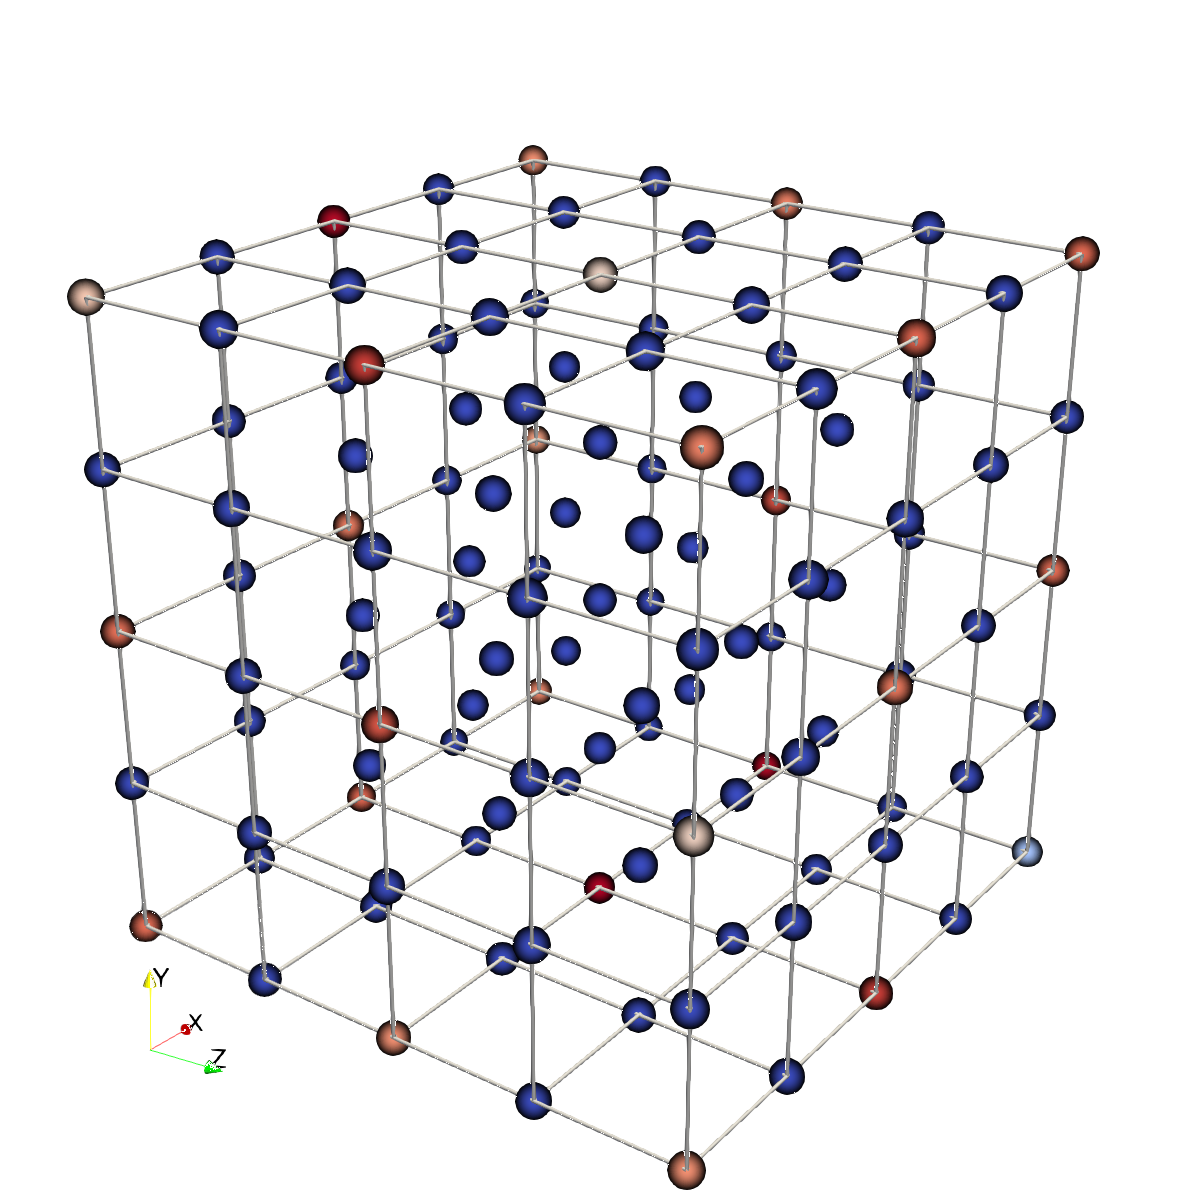
\includegraphics[width=0.6\linewidth]{stream_2.png}
  \end{center}
\end{columns}
\end{frame}


